\newcommand{\lecturetitle}[1]{
  \title{01204211 Discrete Mathematics \\ #1}
  \author{Jittat Fakcharoenphol}
  \frame{\titlepage}
}

\lecturetitle{Lecture 14: Binomial Coefficients (2)} 

\begin{frame}\frametitle{The binomial coefficients\footnote{This lecture mostly follows Chapter 3 of [LPV].}}
  In this lecture, we shall study the function $\binom{n}{k}$ itself.
  First, let's see the actual value of the binomial coefficients
  $\binom{n}{k}$ for various values of $n$.
  \vspace{2in}
\end{frame}

\begin{frame}\frametitle{What do you see?}
  \begin{itemize}
  \item The function $\binom{n}{\cdot}$ is symmetric around $n/2$.
  \item Why? \pause This is true because we know that $\binom{n}{k}=\binom{n}{n-k}$. \pause
  \item The maximum is at the middle, i.e., when $n$ is even the
    maximum is at $\binom{n}{n/2}$ and when $n$ is odd, the maximum is
    at $\binom{n}{\lfloor n/2 \rfloor}$ and $\binom{n}{\lceil
      n/2\rceil}$.
  \item Why? \pause Can we prove that?
  \end{itemize}
\end{frame}

\begin{frame}\frametitle{Largest in the middle}
  To understand the behavior of $\binom{n}{k}$ as $k$ changes, let's
  look at two consecutive values:
  \[ \binom{n}{k} \ \ \heartsuit \ \ \binom{n}{k+1}\]
  \pause

  Let's write them out:
  \[ \frac{n(n-1)(n-2)\cdots(n-k+1)}{k!} \ \heartsuit \ \frac{n(n-1)(n-2)\cdots(n-k)}{(k+1)k!}.\]
  \pause
  Removing common terms, we can see that we are comparing these two terms:
  \[ 1 \ \heartsuit \ \frac{n-k}{k+1} \Leftrightarrow k \ \heartsuit \ \frac{n-1}{2},\]
  that is, \pause
  \begin{itemize}
  \item if $k<(n-1)/2$, $\binom{n}{k} < \binom{n}{k+1}$; and
  \item if $k>(n-1)/2$, $\binom{n}{k} > \binom{n}{k+1}$.
  \end{itemize}
\end{frame}

\begin{frame}\frametitle{How large is the middle $\binom{n}{n/2}$}
  Here, to simplify the calculation, we shall only consider the case
  when $n$ is even. Let's try to estimate the value of
  $\binom{n}{n/2}$ by finding its upper and lower bounds.
  \pause

  A simple upper bound can be obtain using the fact that
  $\binom{n}{n/2}$ counts subsets of certain size:
  \[\binom{n}{n/2} < 2^n.\]
  \pause

  We can also get a lower bound by noting that the maximum must be at
  least the average, i.e.,
  \[\binom{n}{n/2} \geq \frac{2^n}{n+1}\]
\end{frame}

\begin{frame}
  Combining both bounds, we get that
  \[\frac{2^n}{n+1}\leq \binom{n}{n/2} < 2^n.\]

  \pause Let's plug in $n=200$, and calculate the number of digits to
  see how close these bounds.
  \[27.80 \approx 200\cdot\log 2 - \log 201 \leq \log\binom{n}{n/2} < 200\cdot \log 2\approx 30.10\]
  \pause

  Can we get a better approximation? \pause

  Yes, with Stirling's formula. (homework)
\end{frame}

\begin{frame}\frametitle{Concentration}
  \begin{itemize}
  \item We know that the maximum of $\binom{n}{k}$ is obtained when
    $k=n/2$.  From the graph, you can see that, as you move further
    from the middle, the value of the function drops rapidly.
  \item Since we consider even $n$, we let $2m=n$.  One way to
    quantify how fast the values drop is to think about the ratio
    \[ \binom{2m}{m-t}\Big/\binom{2m}{m}. \] \pause
  \item In fact, it is known that
    \[ \binom{2m}{m-t}\Big/\binom{2m}{m} \approx e^{-t^2/m} \]
    \pause
  \item We will use our basic tools to obtain weaker bounds.
  \end{itemize}
\end{frame}

\begin{frame}\frametitle{How close is the approximation?}
  The estimation $e^{-t^2/m}$ is extremely close as shown in the
  figure below, where the gray bars are the actual value of
  $\binom{2m}{m-t}/\binom{2m}{m}$ and the red line is $e^{-t^2/m}$.

  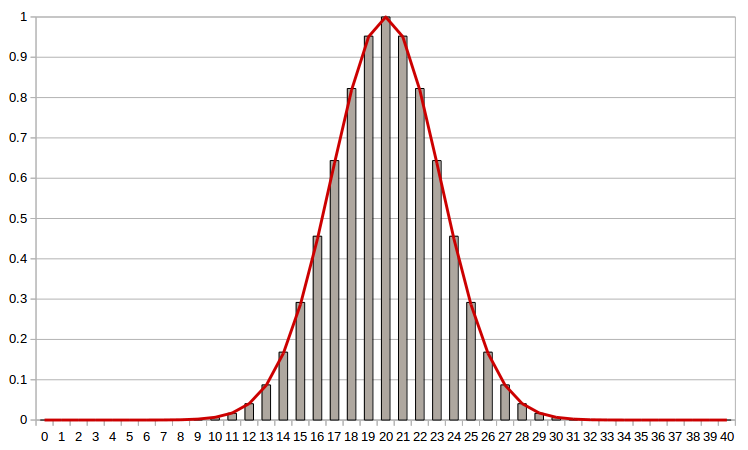
\includegraphics[height=2.2in]{images/binom-approx.png}
\end{frame}

\begin{frame}\frametitle{The actual values}
  Because dealing with numbers less than 1 with logarithms is
  error-prone, we will work on the reciprocal.  Let's try to calculate
  the ratio
  \begin{eqnarray*}
    \binom{2m}{m}\Big/\binom{2m}{m-t}
    &=&
    \frac{(2m)!}{m!m!}\times\frac{(2m-m+t)!(m-t)!}{(2m)!}\\
    &=&
    \frac{(m+t)(m+t-1)\cdots(m+1)}{m(m-1)(m-2)\cdots(m-t+1)}.
  \end{eqnarray*}
  \pause
  We can use the same logarithm trick.  We have that the log of the
  ratio is
  \[
  \ln\left(\frac{m+t}{m}\right) +
  \ln\left(\frac{m+t-1}{m-1}\right)+\cdots+
  \ln\left(\frac{m+1}{m-t+1}.\right).
  \]
  \pause
  Then we can apply the bounds we have for $\ln x$:
  \[
  \frac{x-1}{x}\leq \ln x \leq x - 1
  \]
\end{frame}

\begin{frame}\frametitle{The upper bound on the reciprocal}
  Each term in the sum is in this form $\ln((m-i)/(m+t-i))$.  Applying
  the upper bound, we get
  \[ \ln\left(\frac{m+t-i}{m-i}\right) \leq \frac{m+t-i}{m-i}-1 = \frac{m+t-i-m+i}{m-i}=\frac{t}{m-i}.\]
  \pause

  Let's sum them up to get
  \[
    \ln\left(\frac{m+t}{m}\right) +
    \ln\left(\frac{m+t-1}{m-1}\right)+\cdots+
    \ln\left(\frac{m+1}{m-t+1}.\right) \quad\quad\quad
  \]
  \begin{eqnarray*}
    \quad\quad &\leq&
    \frac{t}{m} + \frac{t}{m-1} + \cdots + \frac{t}{m-t+1} \\
    &\leq&
    \frac{t}{m-t+1} + \frac{t}{m-t+1} + \cdots + \frac{t}{m-t+1} \\
    & = & \frac{t^2}{m-t+1}. \\
  \end{eqnarray*}
\end{frame}

\begin{frame}
  This implies that
  \[
  \ln\left(\frac{(m+t)(m+t-1)\cdots(m+1)}{m(m-1)(m-2)\cdots(m-t+1)}\right)
  \leq \frac{t^2}{m-t+1},
  \]
  i.e.,
  \begin{eqnarray*}
    \binom{2m}{m}\Big/\binom{2m}{m-t} &=& 
    \left(\frac{(m+t)(m+t-1)\cdots(m+1)}{m(m-1)(m-2)\cdots(m-t+1)}\right)\\
    &\leq& e^{t^2/(m-t+1)}.
  \end{eqnarray*}
  \pause

  Taking the reciprocal, we get
  \[
  e^{-t^2/(m-t+1)}\leq
  \binom{2m}{m-t}\Big/\binom{2m}{m}.
  \]
\end{frame}

\begin{frame}\frametitle{Upper bounds}
  Using the same approach, we can show that
  \[
  \binom{2m}{m-t}\Big/\binom{2m}{m}\leq e^{-t^2/(m+t)}.
  \]
  \pause

  Thus, we derived the estimates:
  \begin{tcolorbox}
    \[
    e^{-t^2/(m-t+1)}\leq
    \binom{2m}{m-t}\Big/\binom{2m}{m}
    \leq e^{-t^2/(m+t)},
    \]
  \end{tcolorbox}
  \pause
  which is fairly close the the estimate of $e^{-t^2/m}$.
\end{frame}

\begin{frame}\frametitle{How fast?}
  \begin{itemize}
  \item
    Let's return to the question on how fast do the values of the
    binomial coefficients decrease as you move further from the
    middle.  Let's use the better estimate
    $\binom{2m}{m-t}\big/\binom{2m}{m}\approx e^{-t^2/m}$.  \pause

  \item
    Given a constant $C$, we want to estimate the value of $t$ such
    that $\binom{2m}{m-t}$ is less than $\binom{2m}{m}\big/C$.  (E.g.,
    we can set $C=2$ to see when the value drops by 50\%.) Therefore,
    we want to find $t$ such that
    \[
    1/C \geq 
    \binom{2m}{m-t}\big/\binom{2m}{m}\approx e^{-t^2/m}
    \]
    Taking the logs, we get
    \[
    \ln 1/C = -\ln C \geq 
    \ln \binom{2m}{m-t}\big/\binom{2m}{m}\approx -t^2/m.
    \]
    This is true when
    \[
    t \geq \sqrt{m\ln C}.
    \]
  \end{itemize}
\end{frame}

\begin{frame}\frametitle{What does this means?}
  As an example, let $m=20$ and $C=2$.  We know that when $t$ is
  approximately $\sqrt{20\cdot \ln 2} = 3.723$ the value of
  $\binom{2m}{m-t}$ drops by 50\%.

  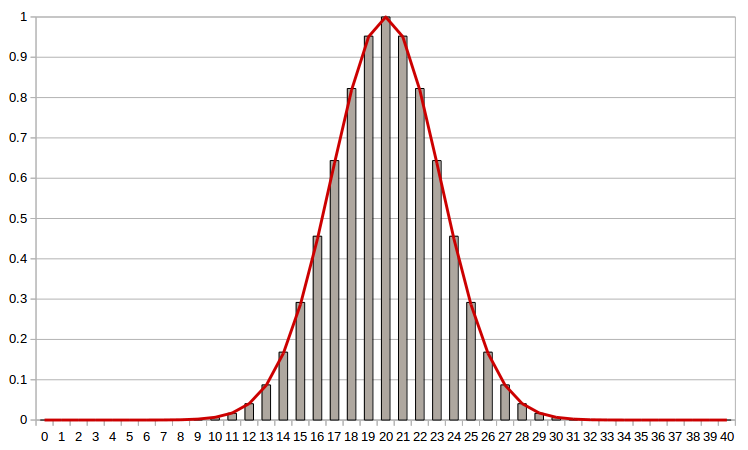
\includegraphics[height=2.2in]{images/binom-approx.png}

\end{frame}
